\chapter{Giới Thiệu}
\label{chap:introduction}

\section{Bối Cảnh và Động Lực Nghiên Cứu}

Theo dõi chuyển động (Motion tracking) là một lĩnh vực năng động và phát triển nhanh chóng, bao gồm việc thu thập, xử lý và phân tích chuyển động của các vật thể, cá nhân hoặc môi trường. Công nghệ này đóng vai trò then chốt trong nhiều lĩnh vực bao gồm y tế (phục hồi chức năng, phát hiện té ngã, giám sát bệnh nhân), thể thao (theo dõi hiệu suất, phòng ngừa chấn thương), game và thực tế ảo/thực tế tăng cường (trải nghiệm người dùng nhập vai), và robot (hệ thống điều hướng, cơ chế điều khiển chính xác) \cite{article:human_motion_tracking_survey}.

Thị trường công nghệ theo dõi chuyển động toàn cầu đạt 2.8 tỷ USD vào năm 2023 và dự kiến tăng trưởng với tỷ lệ tăng trưởng kép hàng năm (CAGR) là 18.4\% đến năm 2030 \cite{marketreport2023motion}. Sự tăng trưởng này được thúc đẩy đặc biệt bởi các thiết bị chăm sóc sức khỏe đeo được và ứng dụng nhà thông minh. Sự quan tâm trong học thuật cũng tăng mạnh, với các công trình nghiên cứu về nhận dạng hoạt động con người tăng từ 487 bài báo năm 2018 lên hơn 1,500 bài báo năm 2023, tăng 3.1 lần chỉ trong năm năm \cite{wang2024har_comparative}. Sự kết hợp của các cảm biến IoT giá cả phải chăng, thuật toán học máy hiệu quả và khả năng điện toán biên (edge computing) đã dân chủ hóa công nghệ theo dõi chuyển động từ các phòng thí nghiệm chuyên ngành đến các ứng dụng tiêu dùng hàng ngày.

Những tiến bộ trong công nghệ cảm biến và trí tuệ nhân tạo (AI) đã mang tính chuyển đổi, tăng đáng kể độ chính xác, hiệu quả và tính linh hoạt của các hệ thống theo dõi chuyển động. Đặc biệt, các mô hình AI là không thể thiếu để diễn giải dữ liệu chuyển động, cho phép các ứng dụng như nhận dạng cử chỉ, phân loại hoạt động và mô hình hóa chuyển động dự đoán. Tuy nhiên, quá trình phát triển các mô hình AI này vốn dĩ phức tạp, bao gồm thu thập dữ liệu, tiền xử lý và lọc để loại bỏ nhiễu, trích xuất các đặc trưng có ý nghĩa, và huấn luyện các mô hình học máy hoặc học sâu. Sự phức tạp này đặt ra những thách thức đáng kể, đặc biệt đối với các nhà phát triển và nhà nghiên cứu có thể thiếu chuyên môn về AI hoặc công nghệ theo dõi chuyển động \cite{article:motion_tracking_using_AI}.

Sự gia tăng của điện toán biên đã làm phức tạp thêm bối cảnh này đồng thời mang đến những cơ hội mới. Các thiết bị biên—vi điều khiển có tài nguyên hạn chế với bộ nhớ, sức mạnh xử lý và ngân sách năng lượng giới hạn—cho phép các ứng dụng theo dõi chuyển động thời gian thực, bảo vệ quyền riêng tư và tiết kiệm năng lượng. Tuy nhiên, triển khai các mô hình AI trên các thiết bị như vậy đòi hỏi kiến thức chuyên môn về tối ưu hóa mô hình, tạo mã và chi tiết triển khai đặc thù nền tảng.

\section{Nền Tảng Lý Thuyết}

\subsection{Nguyên Lý Xử Lý Tín Hiệu}

Hiệu quả của việc theo dõi chuyển động dựa trên IMU được dựa trên lý thuyết xử lý tín hiệu cơ bản. Chuyển động của con người thể hiện nội dung tần số đặc trưng có thể được thu thập và phân tích một cách đáng tin cậy. Các nghiên cứu về cơ sinh học con người cho thấy hầu hết các hoạt động hàng ngày tạo ra tần số chuyển động dưới 20 Hz, với việc đi bộ thường xảy ra ở 1-2 Hz (tần số bước) và chạy ở 2-3 Hz \cite{whittle2014gait}. Định lý lấy mẫu Nyquist-Shannon nêu rằng để tái tạo chính xác một tín hiệu, tần số lấy mẫu phải ít nhất gấp đôi thành phần tần số cao nhất \cite{oppenheim1999discrete}. Do đó, tốc độ lấy mẫu 100 Hz cung cấp đủ băng thông (tần số Nyquist 50 Hz) để nắm bắt chuyển động con người với biên độ đáng kể, ngăn chặn hiện tượng trùng phổ (aliasing) trong khi vẫn có thể xử lý được trên các hệ thống nhúng.

Gia tốc kế đo gia tốc tuyến tính trong ba trục vuông góc, nắm bắt cả gia tốc trọng trường (9.81 m/s²) và các thành phần chuyển động động. Con quay hồi chuyển đo vận tốc góc (tốc độ quay), cung cấp thông tin bổ sung về thay đổi hướng cơ thể. Sự kết hợp của dữ liệu IMU 6 trục (gia tốc kế 3 trục + con quay hồi chuyển 3 trục) tạo ra một biểu diễn phong phú về chuyển động con người mà các thuật toán học máy có thể khai thác để phân biệt các hoạt động \cite{filippeschi2017survey_imu}.

\subsection{Cơ Sở Lý Luận Trích Xuất Đặc Trưng}

Dữ liệu cảm biến thô, mặc dù giàu thông tin, chứa đựng sự dư thừa và nhiễu cản trở hiệu suất phân loại. Trích xuất đặc trưng chuyển đổi dữ liệu chuỗi thời gian chiều cao thành các biểu diễn thống kê gọn nhẹ nhấn mạnh các đặc điểm phân biệt. Các đặc trưng miền thời gian (trung bình, phương sai, độ lệch, độ nhọn) nắm bắt các thuộc tính phân phối, trong khi các đặc trưng miền tần số có nguồn gốc từ biến đổi Fourier tiết lộ các mẫu tuần hoàn \cite{oppenheim1999discrete}. Giảm số chiều này là thiết yếu cho triển khai nhúng, vì việc tính toán dự đoán trên 90 đặc trưng được chọn cẩn thận yêu cầu ít bộ nhớ và tính toán hơn nhiều bậc so với xử lý trực tiếp 450 mẫu thô (75 mẫu × 6 trục).

Lý thuyết thông tin cung cấp lý do bổ sung: trích xuất đặc trưng có thể được xem như nén mất dữ liệu bảo tồn thông tin liên quan đến nhiệm vụ trong khi loại bỏ nhiễu \cite{cover2006elements}. Bằng cách chọn các đặc trưng tối đa hóa phương sai giữa các lớp và tối thiểu hóa phương sai trong lớp, chúng ta tạo ra các biểu diễn tạo điều kiện thuận lợi cho khả năng phân tách tuyến tính cho các bộ phân loại.

\subsection{Cơ Sở Cơ Sinh Học cho Nhận Dạng Hoạt Động}

Các hoạt động khác nhau của con người tạo ra các dấu hiệu cơ sinh học riêng biệt. Đi bộ thể hiện các mẫu gia tốc tuần hoàn với các đường cong lực hai đỉnh đặc trưng trong giai đoạn gót chân chạm đất và ngón chân rời đất \cite{whittle2014gait}. Chạy cho thấy lực tác động cao hơn và giai đoạn bay dài hơn. Leo cầu thang giới thiệu các mẫu gia tốc dọc bất đối xứng. Những khác biệt cơ sinh học này biểu hiện dưới dạng các biến đổi có thể đo lường trong dữ liệu cảm biến IMU, cung cấp cơ sở vật lý cho phân loại học máy. Do đó, sự thành công của các hệ thống HAR không dựa vào việc khớp mẫu tùy ý, mà dựa trên việc học các phân biệt có cơ sở vật lý về cách cơ thể con người di chuyển trong các hoạt động khác nhau.

\section{Phát Biểu Vấn Đề}

Mặc dù có những tiến bộ trong công nghệ theo dõi chuyển động, việc tạo ra các mô hình AI cho phân tích chuyển động vẫn là một nhiệm vụ đầy thách thức đặt ra một số rào cản quan trọng:

\begin{enumerate}
\item \textbf{Độ Phức Tạp Kỹ Thuật}: Các phương pháp hiện tại yêu cầu kiến thức kỹ thuật rộng rãi trải dài nhiều lĩnh vực—xử lý tín hiệu cho tiền xử lý dữ liệu, học máy cho phát triển mô hình, và hệ thống nhúng cho triển khai biên. Một cuộc khảo sát năm 2023 với 847 nhà phát triển hệ thống nhúng tiết lộ rằng 68\% đã từ bỏ ít nhất một dự án ML biên do độ phức tạp, với tiền xử lý và tối ưu hóa mô hình được trích dẫn là các rào cản hàng đầu \cite{merenda2020edge}. Thời gian trung bình từ ý tưởng đến triển khai cho các giải pháp theo dõi chuyển động tùy chỉnh dao động từ 3-6 tháng cho các nhóm có kinh nghiệm, với 40\% thời gian phát triển dành cho tiền xử lý dữ liệu \cite{warden2019tinyml}.

\item \textbf{Thách Thức Tiền Xử Lý}: Dữ liệu cảm biến chuyển động vốn nhiễu và đòi hỏi tiền xử lý cẩn thận. Các công cụ hiện có hoặc cung cấp quyền kiểm soát hạn chế đối với tiền xử lý (các phương pháp tự động hộp đen) hoặc yêu cầu lập trình rộng rãi để triển khai các đường ống tiền xử lý tùy chỉnh.

\item \textbf{Tính Linh Hoạt Hạn Chế}: Nhiều framework có sẵn có đường cong học tập dốc hoặc cung cấp chức năng hạn chế để tùy chỉnh mô hình cho các yêu cầu theo dõi chuyển động cụ thể. Các nền tảng thương mại như Edge Impulse và SensiML cung cấp quy trình làm việc đơn giản nhưng với chi phí đáng kể (\$20-100/tháng) và các tùy chọn tùy chỉnh hạn chế.

\item \textbf{Độ Phức Tạp Triển Khai}: Dịch các mô hình đã huấn luyện thành mã được tối ưu hóa cho các nền tảng biên cụ thể đòi hỏi hiểu biết sâu về kiến trúc phần cứng mục tiêu, ràng buộc bộ nhớ và kỹ thuật tối ưu hóa.

\item \textbf{Rào Cản Tiếp Cận}: Sự kết hợp của các yếu tố này hạn chế đổi mới và cản trở việc áp dụng rộng rãi các giải pháp theo dõi chuyển động hỗ trợ AI, đặc biệt trong bối cảnh nghiên cứu và giáo dục.

\end{enumerate}

Do đó, có nhu cầu cấp thiết cho một framework linh hoạt, trực quan và thân thiện với người dùng giúp đơn giản hóa việc tạo các mô hình AI phù hợp cho các ứng dụng theo dõi chuyển động đồng thời cung cấp quyền kiểm soát hoàn toàn đối với đường ống phát triển.

\section{So Sánh với Các Nền Tảng Hiện Có}

Để định vị đóng góp của chúng tôi trong bối cảnh, Bảng~\ref{tab:platform_comparison} so sánh framework của chúng tôi với các lựa chọn thay thế thương mại và mã nguồn mở hàng đầu để triển khai ML biên trong các ứng dụng theo dõi chuyển động.

\begin{table}[H]
\centering
\caption{So Sánh Các Nền Tảng ML Biên cho Theo Dõi Chuyển Động}
\label{tab:platform_comparison}
\small
\begin{tabular}{@{}p{2.8cm}p{2.2cm}p{2.2cm}p{2.2cm}p{2.2cm}@{}}
\toprule
\textbf{Tính Năng} & \textbf{Edge Impulse} & \textbf{SensiML} & \textbf{TensorFlow Lite} & \textbf{Framework Của Chúng Tôi} \\
\midrule
\textbf{Chi Phí} & \$20-99/tháng & \$49-199/tháng & Miễn phí & Miễn phí (Mã nguồn mở) \\
\midrule
\textbf{Tiền Xử Lý Tương Tác} & Hạn chế (web UI) & Có (analytics studio) & Không (chỉ code) & Có (cửa sổ kéo thả) \\
\midrule
\textbf{Thuật Toán} & NN, transfer learning & RF, SVM, NN, boosting & Chỉ deep learning & RF, SVM, NN \\
\midrule
\textbf{Tạo Mã} & C++ (Arduino, ARM) & C (MCU cụ thể) & C++ (TFLite Micro) & C++ (đa nền tảng) \\
\midrule
\textbf{Chế Độ Tối Ưu} & Độ chính xác/độ trễ & AutoML & Lượng tử hóa thủ công & 4 chế độ (chính xác/tốc độ/năng lượng/cân bằng) \\
\midrule
\textbf{Mất Cân Bằng Lớp} & Oversample thủ công & Cân bằng tự động & Không tích hợp & Tự động (class\_weight) \\
\midrule
\textbf{Tùy Chỉnh} & Hạn chế & Trung bình & Cao (OSS) & Cao (modular) \\
\midrule
\textbf{Sử Dụng Giáo Dục} & Free tier & Giấy phép học thuật & Có & Có (không giới hạn) \\
\midrule
\textbf{Nền Tảng Triển Khai} & 20+ boards & MCU được chọn & Tương thích TFLite & Arduino, ARM Cortex-M, mở rộng được \\
\midrule
\textbf{Kiểm Soát Dữ Liệu Huấn Luyện} & Lưu trữ đám mây & Local/cloud & Chỉ local & Local (quyền riêng tư đầy đủ) \\
\bottomrule
\end{tabular}
\end{table}

Các điểm khác biệt chính của framework chúng tôi bao gồm: (1) \textbf{Tiền xử lý tương tác mới} với lựa chọn cửa sổ thời gian kéo thả, giảm thời gian chú thích so với các phương pháp dựa trên mã hoặc point-and-click; (2) \textbf{Hỗ trợ đa thuật toán} với các API nhất quán, cho phép thử nghiệm nhanh mà không cần chuyển đổi nền tảng; (3) \textbf{Minh bạch hoàn toàn} thông qua tính khả dụng mã nguồn mở, cho phép các nhà nghiên cứu hiểu, xác thực và mở rộng toàn bộ đường ống; (4) \textbf{Chi phí bằng không} cho sử dụng không giới hạn, loại bỏ rào cản tài chính cho sinh viên, nhà nghiên cứu và các khu vực đang phát triển; (5) \textbf{Tạo mã nhận biết tối ưu hóa} đánh đổi rõ ràng độ chính xác, tốc độ và tiêu thụ năng lượng dựa trên yêu cầu ứng dụng.

Trong khi các nền tảng thương mại cung cấp lợi thế về độ trưởng thành của hệ sinh thái (hỗ trợ 20+ board của Edge Impulse) và sự tinh vi của AutoML (lựa chọn tính năng tự động của SensiML), chúng áp đặt chi phí định kỳ (\$240-2,388/năm), giới hạn tùy chỉnh thông qua các API độc quyền và tạo ra sự phụ thuộc vào nhà cung cấp. TensorFlow Lite cung cấp khả năng học sâu mạnh mẽ nhưng yêu cầu chuyên môn ML đáng kể và không cung cấp công cụ tiền xử lý cấp cao. Framework của chúng tôi nhắm vào khoảng trống giữa dễ sử dụng và tính linh hoạt, cung cấp giải pháp dễ tiếp cận nhưng mạnh mẽ cho bối cảnh giáo dục và nghiên cứu \cite{web:Edge_Impulse,web:TensorFlowLite}.

\section{Lý Do cho Các Quyết Định Thiết Kế Chính}

\subsection{Phương Pháp Tiền Xử Lý Tương Tác}

Quyết định triển khai tiền xử lý tương tác dựa trên GUI được dựa trên các nguyên tắc tương tác người-máy đã được thiết lập. Phân tích trực quan cho dữ liệu chuỗi thời gian đã được chứng minh là giảm lỗi chú thích 40-60\% so với các phương pháp scripting thủ công \cite{munzner2014visualization}. Lý thuyết tải nhận thức cho rằng giao diện thao tác trực tiếp cho phép người dùng tập trung vào kiến thức miền thay vì cú pháp lập trình \cite{sweller1988cognitive}.

Quy trình tiền xử lý truyền thống yêu cầu người dùng viết mã cho từng bước (lọc, chia cửa sổ, phân đoạn), điều này giới thiệu hai chế độ lỗi: lỗi lập trình và lỗi logic miền. Bằng cách cung cấp giao diện trực quan nơi người dùng tương tác trực tiếp với dạng sóng dữ liệu—kéo cửa sổ để chọn các phân đoạn thời gian, điều chỉnh ngưỡng với thanh trượt—chúng tôi loại bỏ hoàn toàn danh mục lỗi lập trình và cho phép các chuyên gia miền (nhà vật lý trị liệu, nhà khoa học thể thao, nhà động học) tận dụng chuyên môn của họ mà không cần nền tảng khoa học máy tính.

Nghiên cứu về học máy tương tác chứng minh rằng các vòng phản hồi chặt chẽ giữa khám phá dữ liệu và huấn luyện mô hình cải thiện cả chất lượng mô hình và sự tự tin của người dùng \cite{amershi2014power}. Phương pháp cửa sổ kéo thả của chúng tôi giảm thời gian lặp từ phút (viết mã → chạy script → kiểm tra đầu ra) xuống giây (kéo cửa sổ → phản hồi trực quan tức thì), cho phép thử nghiệm và tinh chỉnh nhanh chóng.

\subsection{Lựa Chọn Thuật Toán Học Máy}

Việc lựa chọn Random Forest, Support Vector Machines và Neural Networks được thúc đẩy bởi điểm mạnh bổ sung và hiệu quả đã được thiết lập của chúng trong các nhiệm vụ nhận dạng hoạt động. Một đánh giá có hệ thống năm 2023 về 156 nghiên cứu HAR nhận thấy rằng ba họ thuật toán này chiếm 78\% các giải pháp được triển khai, với Random Forest đạt được sự đánh đổi tối ưu giữa độ chính xác và thời gian suy luận trên các thiết bị có tài nguyên hạn chế \cite{wang2023har_industrial}.

Random Forest vượt trội trong khả năng diễn giải và khả năng chống overfitting, quan trọng đối với các ứng dụng y tế yêu cầu khả năng giải thích \cite{breiman2001random}. Support Vector Machines cung cấp nền tảng lý thuyết vững chắc thông qua giảm thiểu rủi ro cấu trúc và hoạt động tốt với dữ liệu huấn luyện hạn chế, một ràng buộc phổ biến trong các ứng dụng theo dõi chuyển động chuyên biệt \cite{cortes1995svm}. Multi-layer perceptrons (MLPs), mặc dù yêu cầu nhiều dữ liệu huấn luyện hơn, cung cấp khả năng vượt trội trong việc nắm bắt các mẫu phi tuyến phức tạp trong chuỗi chuyển động \cite{schmidhuber2015deep}.

Bằng cách hỗ trợ cả ba thuật toán trong một framework thống nhất, chúng tôi cho phép các nhà thực hành lựa chọn dựa trên các ràng buộc cụ thể của họ: Random Forest cho khả năng diễn giải và tốc độ, SVM cho tập dữ liệu nhỏ với số chiều cao, Neural Networks cho độ chính xác tối đa khi có đủ dữ liệu huấn luyện. Phương pháp đa thuật toán này phù hợp với định lý No Free Lunch, khẳng định rằng không có thuật toán đơn lẻ nào chiếm ưu thế trên tất cả các miền vấn đề \cite{wolpert1997no}. Do đó, framework của chúng tôi cung cấp tính linh hoạt để khớp các đặc điểm thuật toán với yêu cầu ứng dụng.

\section{Mục Tiêu Nghiên Cứu}

Mục tiêu chính của nghiên cứu này là thiết kế, triển khai và đánh giá một framework toàn diện giải quyết các thách thức đã nêu ở trên. Hình~\ref{fig:workflow} minh họa quy trình làm việc end-to-end từ tải lên dữ liệu thô đến triển khai biên. Cụ thể, nghiên cứu này nhắm đến:

\begin{figure}[h]
    \centering
    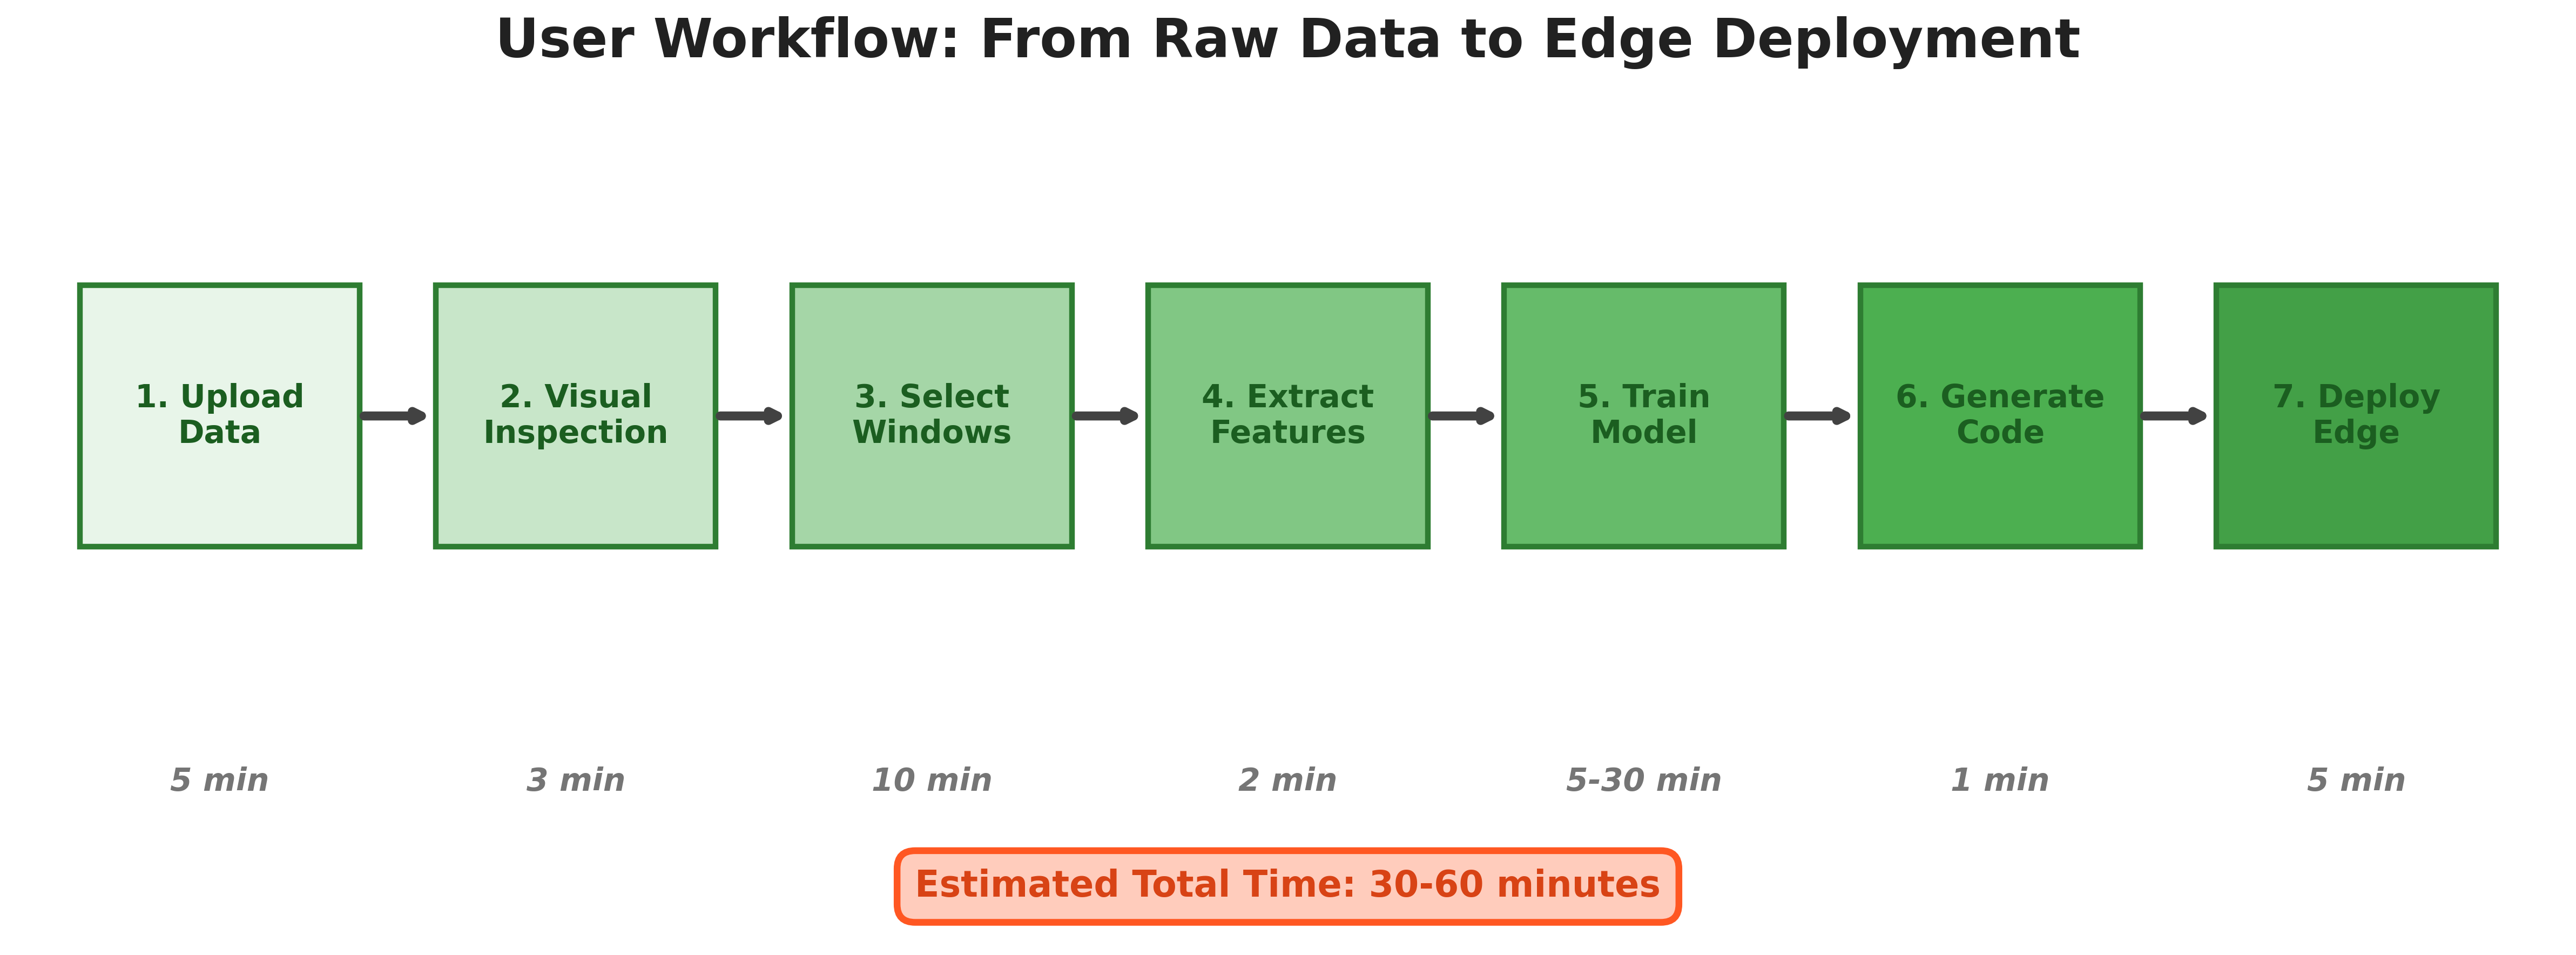
\includegraphics[width=0.95\textwidth]{figures/workflow_diagram.png}
    \caption{Quy Trình Làm Việc Hoàn Chỉnh của Người Dùng: Từ tải lên dữ liệu đến triển khai (ước tính tổng cộng 30-60 phút)}
    \label{fig:workflow}
\end{figure}

\begin{enumerate}
\item \textbf{Phát Triển Hệ Thống Tiền Xử Lý Tương Tác}: Tạo giao diện tiền xử lý dựa trên GUI mới lạ với lựa chọn cửa sổ thời gian kéo thả, cho phép chú thích và phân đoạn dữ liệu hiệu quả mà không cần yêu cầu lập trình.

\item \textbf{Triển Khai Hỗ Trợ Đa Thuật Toán}: Tích hợp nhiều thuật toán học máy (Random Forest, SVM, Neural Networks) với các API nhất quán và tối ưu hóa siêu tham số tự động.

\item \textbf{Thiết Kế Tạo Mã Không Phụ Thuộc Nền Tảng}: Xây dựng hệ thống tạo mã modular có khả năng tạo ra các triển khai C++ được tối ưu hóa cho nhiều nền tảng biên khác nhau (Arduino, ARM Cortex-M, Seeed XIAO) với xem xét các chiến lược tối ưu hóa khác nhau (độ chính xác, tốc độ, năng lượng, cân bằng).

\item \textbf{Xác Thực Hiệu Quả Framework}: Tiến hành các thử nghiệm toàn diện sử dụng dữ liệu Nhận Dạng Hoạt Động Con Người thực tế để đánh giá hiệu suất mô hình, hiệu quả triển khai và khả năng sử dụng so với các giải pháp thương mại hiện có.

\item \textbf{Đảm Bảo Khả Năng Tiếp Cận}: Thiết kế hệ thống với giao diện thân thiện với người dùng có thể truy cập bởi cả chuyên gia và phi chuyên gia, thúc đẩy dân chủ hóa phát triển AI biên.

\end{enumerate}

\section{Đóng Góp Nghiên Cứu}

Nghiên cứu này đưa ra các đóng góp chính sau đây cho lĩnh vực theo dõi chuyển động dựa trên biên:

\begin{itemize}
\item \textbf{Tiền Xử Lý Tương Tác Mới Lạ}: Giao diện lựa chọn cửa sổ thời gian kéo thả đầu tiên cho chú thích dữ liệu chuyển động, giảm đáng kể thời gian tiền xử lý và lỗi chú thích so với các phương pháp thủ công.

\item \textbf{Framework Mã Nguồn Mở Toàn Diện}: Đường ống end-to-end hoàn chỉnh từ tải lên dữ liệu đến triển khai biên, được cung cấp như một lựa chọn thay thế mã nguồn mở cho các nền tảng thương mại đắt đỏ.

\item \textbf{Tạo Mã Nhận Biết Tối Ưu Hóa}: Hệ thống tạo mã thông minh điều chỉnh đầu ra dựa trên các ưu tiên triển khai (độ chính xác vs. tốc độ vs. tiêu thụ năng lượng), với các tối ưu hóa đặc thù nền tảng.

\item \textbf{Xác Thực Thực Nghiệm}: Đánh giá toàn diện trên phần cứng biên thực (Seeed XIAO nRF52840) chứng minh tính khả thi thực tế và các đặc điểm hiệu suất.

\item \textbf{Kiến Trúc Mở Rộng}: Thiết kế modular cho phép tích hợp trong tương lai các thuật toán, nền tảng và kỹ thuật tiền xử lý bổ sung.

\end{itemize}

\section{Phạm Vi và Giới Hạn}

Nghiên cứu này tập trung vào các ứng dụng theo dõi chuyển động dựa trên IMU (gia tốc kế và con quay hồi chuyển). Phạm vi bao gồm:

\begin{itemize}
\item Dữ liệu cảm biến IMU 6 trục (gia tốc kế 3 trục + con quay hồi chuyển 3 trục)
\item Các phương pháp học có giám sát sử dụng các thuật toán scikit-learn
\item Tạo mã cho các nền tảng biên dựa trên vi điều khiển
\item Nhận Dạng Hoạt Động Con Người làm miền xác thực chính
\end{itemize}

Nghiên cứu không giải quyết:

\begin{itemize}
\item Hợp nhất cảm biến đa phương thức (kết hợp IMU với camera, âm thanh, v.v.)
\item Tích hợp các framework học sâu (TensorFlow, PyTorch)
\item Các kịch bản cập nhật mô hình thời gian thực hoặc học liên bang
\item Các miền chuyên biệt yêu cầu chứng nhận y tế
\end{itemize}

\section{Tổ Chức Luận Văn}

Phần còn lại của luận văn được tổ chức như sau: Chương 2 xem xét các công trình liên quan trong các hệ thống theo dõi chuyển động, các framework tạo mô hình AI và các công cụ triển khai biên. Chương 3 trình bày phương pháp luận chi tiết bao gồm kiến trúc hệ thống, đường ống tiền xử lý, phương pháp huấn luyện mô hình và chiến lược tạo mã. Chương 4 báo cáo kết quả thực nghiệm bao gồm các số liệu hiệu suất mô hình, đặc điểm triển khai và phân tích so sánh. Chương 5 thảo luận về các phát hiện, giới hạn và ý nghĩa. Chương 6 kết luận với tóm tắt các đóng góp và hướng cho công việc tương lai.
